% PAKETE UND DOKUMENTKONFIGURATION
\documentclass[11pt, a4paper]{scrbook}

% Encoding für Umlaute
\usepackage[utf8]{inputenc}
\usepackage[T1]{fontenc}

% Silbentrennung
\usepackage[ngerman]{babel}

% erweiterte Matheumgebungen und Formelnummer mit Sectionnummer
\usepackage{amsmath}

% zusätzliche mathematische Schriftarten
\usepackage{amsfonts}

% verschiedene mathematische Symbole
\usepackage{amssymb}

% Einheiten setzen z.B. \SI{10}{\kilo\gram\meter\per\second\squared}
% Fehler: \SI{10 +- 0,2e-4}{\metre}
\usepackage{siunitx}
\sisetup{
  output-decimal-marker={,},
  separate-uncertainty
}

% Bilder einfügen
\usepackage{graphicx}

% Textfarbe
\usepackage[dvipsnames]{xcolor}

% Verweise innerhalb des Dokuments
\usepackage{hyperref}
\hypersetup{
	colorlinks = true,
	allcolors = {black}
}

\newcommand{\vnabla}{\vec{\nabla}}
\newcommand{\ve}{\vec{E}}
\newcommand{\vb}{\vec{B}}
\newcommand{\vh}{\vec{H}}
\newcommand{\vd}{\vec{D}}

\newcommand{\todo}[1]{{\textcolor{Green}{(#1)}}}

\title{Störkörpermessung an Beschleunigungsresonatoren}
\author{Christopher Deutsch}

\begin{document}
	\frontmatter
	\maketitle
	\tableofcontents
	
	\mainmatter
	
	\chapter{Einleitung}
	
	
	\chapter{Theorie}
	Kavitäten -> Beschleunigen Teilchen
	Beschleunigung benutzt Hochfrequenz -> EM-Wellen -> Hohlleiter / Cavities\\
	Beschleunigung durch travelling wave nicht möglich -> Randbedingung (Leiter) muss existieren um Feld in Propagationsrichtung der Welle zu bekommen (Hohlleiter).
	Beschleunigung in Hohlleitern ebenfalls nicht möglich da die Phasengeschwindigkeit der EM-Welle in Hohlleitern größer ist als Lichtgeschwindigkeit.
	[WIEDEMANN] Reduzierung der Phasengeschwindigkeit (traveling wave linac structures) oder Ausbilden von stehenden Wellen (single accelerating cavities)
	
	Resonanzüberhöhung, Hohlraumresonatoren, Schwingung angeregt ausgeprägtes (longitudinales) Feld TM010\\
	Oftmals Kette mehrerer Zellen (Phase?), Kopplung durch Irisblenden.
	Modell: Durch Irisblenden belasteter Hohlleiter. (Stehwellenresonator)
	Oft benutzt für Elektronen $\beta = 1$: \url{https://cas.web.cern.ch/cas/Denmark-2010/Lectures/Gerigk.pdf}
	(konstante Zellenlänge).
	
	Randbedingungen: tangential $\ve$ und normal $\vb$ muss verschwinden.
	
	$TM_{mnp}, TE_{mnp}$:\\
	$m$ volle Perioden der Feldkomponenten in azimutaler Richtung\\
	$n$ Anzahl der Knoten der longitudinalen Feldkomponente in der radialen Richtung (ohne $r=0$)\\
	$p$ halbe Perioden der Feldkomponenten in longitudinaler Richtung
	
	\section{Hohlraumresonatoren}
	Ein Hohlraumresonator besteht aus einem evakuierten Hohlraum, welcher durch ein leitendes Material begrenzt wird.
	Die im Hohlraum propagierenden elektromagnetischen Wellen werden an den leitenden Wänden reflektiert und führen zur Ausbildung von stehenden elektromagnetischen Wellen im Resonatorinnenraum, welche unter anderem zur Beschleunigung von elektrisch geladenen Teilchen genutzt werden können.
	Aufgrund der Randbedingungen an der leitenden Grenzfläche müssen die folgenden Anforderungen an das elektromagnetische Feld gestellt werden:
	\begin{align}
		E_\parallel = 0 \qquad \text{und} \qquad B_\perp = 0\text{,}
	\end{align}
	wobei $E_\parallel$ die Tangentialkomponente und $B_\perp$ die Normalkomponente des elektrischen bzw.\ magnetischen Feldes auf der Grenzfläche kennzeichnet.
	Die Lösung der \textsc{Maxwell}-Gleichungen unter Beachtung dieser Grenzbedingungen zeigt, dass in Abhängigkeit der Geometrie des Hohlraums, nur gewisse Moden mit bestimmten Frequenzen im Resonator auftreten können.
	Die Klassifizierung der einzelnen Moden erfolgt dabei anhand ihrer Feldkonfiguration relativ zur Propagationsrichtung der hin- beziehungsweise rücklaufenden Wellen im Resonator.
	Dabei unterscheidet man zwischen transversal elektrischen (TE)-Moden, welche lediglich transversale elektrische und longitudinal magnetische Felder aufweisen und transversal magnetischen (TM)-Moden, bei denen der umgekehrte Fall eintritt.
	\cite{wangler}:
	\begin{subequations}
		\begin{align}
		\text{TM-Moden:} \quad E_z = E_0 J_m(k_{mn} r) \cos(m \theta) \cos\left(\frac{p \pi z}{l}\right) \exp(i \omega_{mnp} t) \qquad B_z = 0\\
		\text{TE-Moden:} \quad E_z = 0 \qquad B_z = B_0 J_m(k_{mn}^\prime r) \cos(m \theta) \sin\left(\frac{p \pi z}{l}\right) \exp(i \omega_{mnp} t)
		\end{align}
	\end{subequations}

	\begin{align}
	k_{mn} = \frac{x_{mn}}{R}
	\end{align}
	mit Radius $R$ und Nullstelle $x_{mn}$ die $n$-te Nullstelle ($>0$) der Besselfunktion $J_m$ beziehungsweise $x_{mn}^\prime$ deren Ableitung.
	
	
	
	\section{Hohlraumresonatoren2}
	\begin{figure}[h]
		\centering
		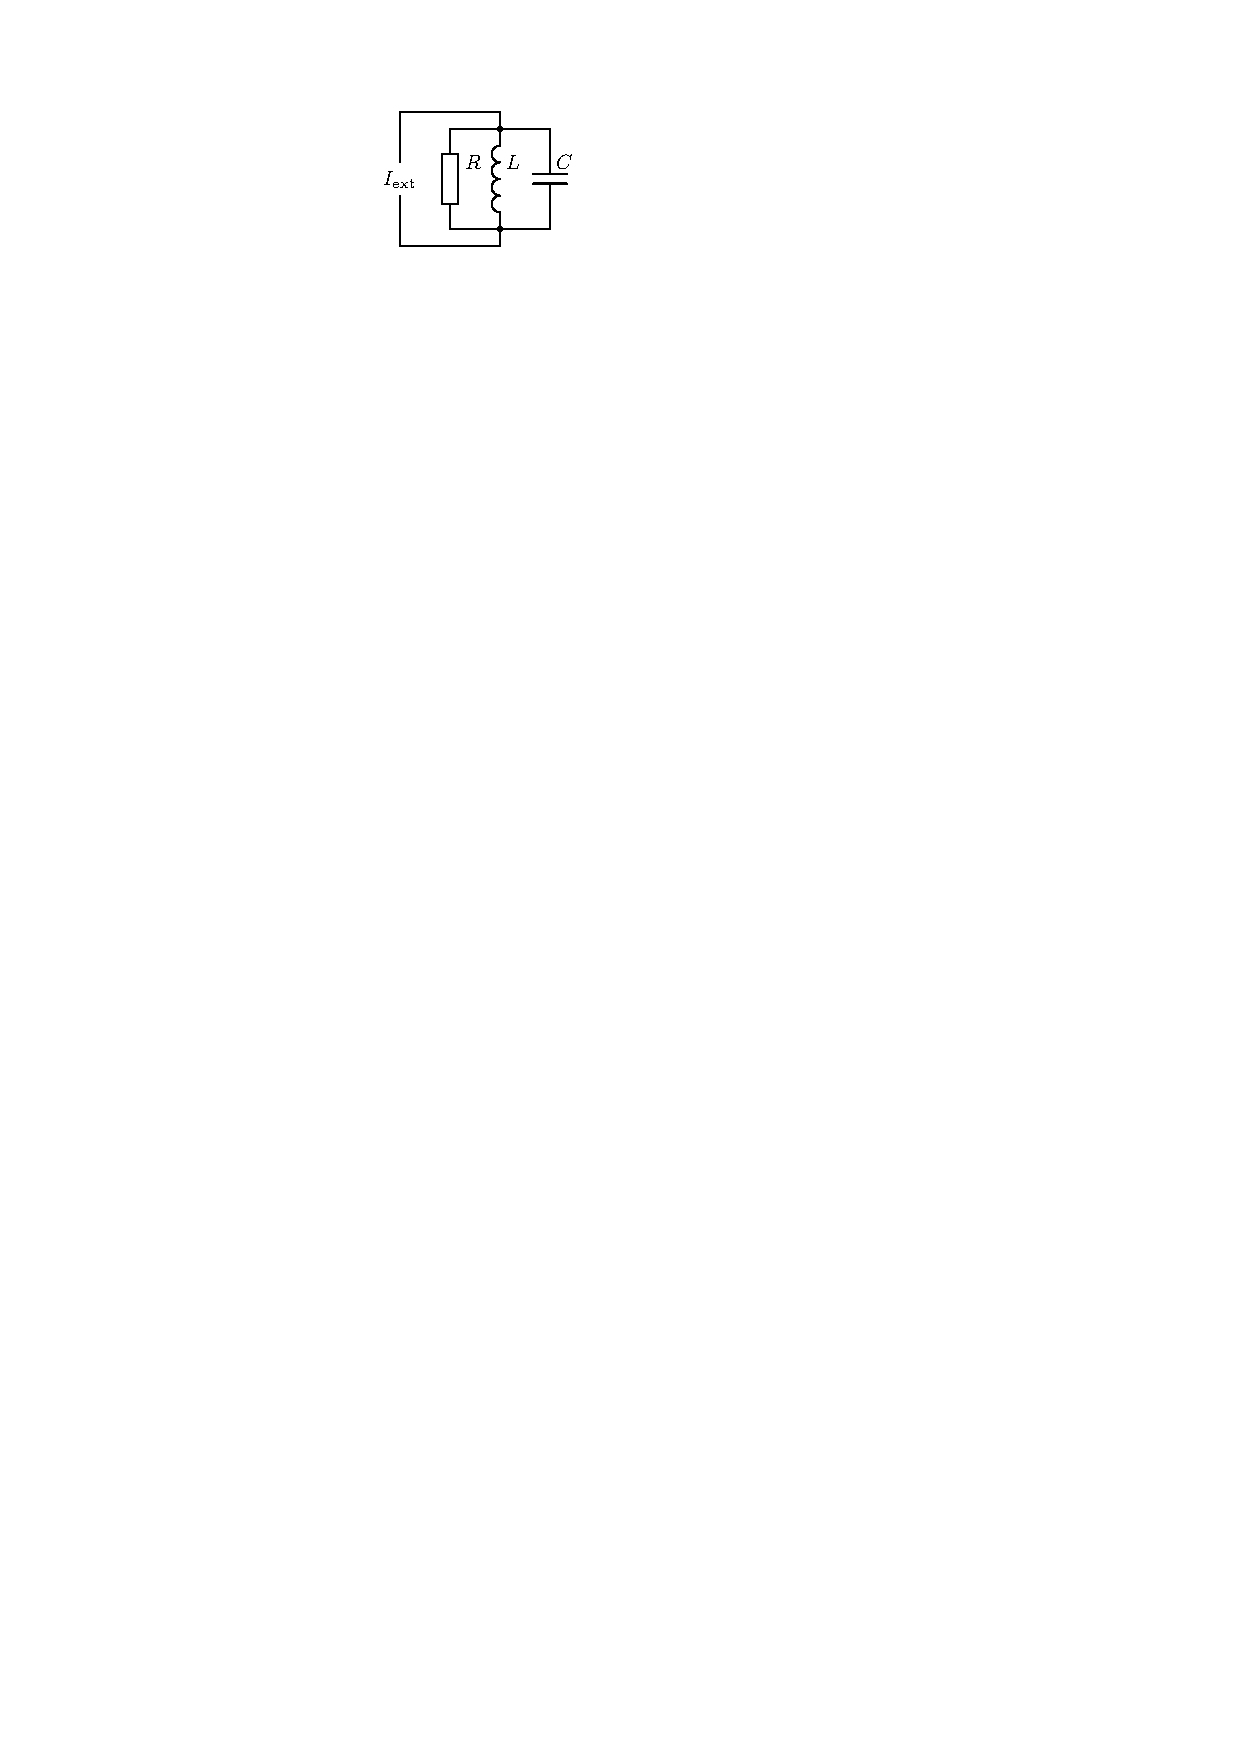
\includegraphics[width=0.35\textwidth]{./figures/RLC_circuit.pdf}
		\caption{RLC Parallelschwingkreis}
		\label{fig:rlc_circuit}
	\end{figure}
	Die elektrischen Eigenschaften von Hohlraumresonatoren in der Nähe einer Resonanz können durch das Modell eines Parallelschwingkreises erklärt werden.
	Die Resonanzfrequenz ist gegeben durch die Thomson'sche Schwingungsgleichung:
	\begin{align}
		\omega_0 = \frac{1}{\sqrt{L C}}
	\end{align}
	(Güte)
	Die Impedanz des Schwingkreises ist gegeben durch:
	\begin{align}
		Z_\mathrm{LCR} = \left( \frac{1}{R} + \frac{1}{i \omega L} + i \omega C \right)^{-1}
	\end{align}
	Unter der Verwendung der Ausdrücke von Resonanzfrequenz und Güte kann dies geschrieben werden als:
	\begin{align}
		Z_\mathrm{LCR} = \frac{R}{1 + i Q_0 \left( \frac{\omega}{\omega_0}  - \frac{\omega_0}{\omega}\right)}
	\end{align}
	(Maybe Phasensprung, im fall von resonanz reell)
	Durch die magnetische Kopplung wird die Impedanz des Resonators transformiert und wird beschrieben durch:
	\begin{align}
		\kappa = \frac{Z^\prime(\omega_0)}{Z_0}
	\end{align}
	($\kappa < 1$ unterkritisch, $\kappa = 0$ kritisch, $\kappa > 1$ überkritisch)
	wobei $Z^\prime$ die transformierte Impedanz ist und $Z_0$ der Wellenwiderstand des Wellenleiters.
	Ebenfalls wird die zusätzliche Impedanz des Leiters in den Resonator transformiert, was die Güte des Gesamtsystems verändert:
	\begin{align}
		\frac{1}{Q} = \frac{1}{Q_0} + \frac{1}{Q_\mathrm{ext}} \\
		Q_0 = (1 + \kappa) \cdot Q
	\end{align}
	Im folgenden ist der komplexe Reflexionsfaktor $\rho$ von besonderem Interesse:
	\begin{align}
		\rho = \frac{U_{-}}{U_{+}} = \frac{Z^\prime - Z_0}{Z^\prime + Z_0}
	\end{align}
%	($Z^\prime$ transformierte Impedanz, $Z_0$ Wellenwiderstand)
	Es folgt für den Reflexionsfaktor
	\begin{align}
		\rho(\omega) = \frac{(\kappa - 1) + i  Q_0 \left( \frac{\omega}{\omega_0}  - \frac{\omega_0}{\omega}\right)}{\left( \kappa + 1 \right) + i  Q_0 \left( \frac{\omega}{\omega_0}  - \frac{\omega_0}{\omega}\right)}
	\end{align}
	Mit dem Betrag:
	\begin{align}
		| \rho(\omega) | = \sqrt{\frac{(\kappa - 1)^2 + Q_0^2 \left( \frac{\omega}{\omega_0}  - \frac{\omega_0}{\omega}\right)^2}{(\kappa + 1)^2 + Q_0^2 \left( \frac{\omega}{\omega_0}  - \frac{\omega_0}{\omega}\right)^2}}
	\end{align}
	Damit ist die vom Resonator aufgenommene Leistung:
	\begin{align}
		P_\mathrm{a} = P_0 (1- |\rho|^2)
	\end{align}
	\section{Resonante Störkörpermessung}
	Feld der ungestörten Cavity $\ve_0$ und der gestörten $\ve_1$:
	\begin{subequations}
		\begin{align}
		&\ve_{0,1}(x,y,z,t) = \ve_{0,1}(x,y,z) \, e^{i \omega t} \\
		&\vh_{0,1}(x,y,z,t) = \vh_{0,1}(x,y,z) \, e^{i \omega t}
		\end{align}
	\end{subequations}
	wobei im folgenden mit nur mit den komplexen Amplituden gerechnet wird.
	Mit den Maxwell-Gleichungen:
	\begin{subequations}
		\begin{align}
			&\vnabla \times \ve = - \frac{\partial \vb}{\partial t} \\
			&\vnabla \times \vh = \frac{\partial \vd}{\partial t}
		\end{align}
	\end{subequations}
	folgt nach Elimination der Zeitabhängigkeit:
	\begin{subequations}
		\begin{align}
			&\vnabla \times \ve_{0,1} = - i \omega_{0,1} \vb_{0,1} \\
			&\vnabla \times \vh_{0,1} = i \omega_{0,1} \vd_{0,1}
		\end{align}
	\end{subequations}
	Unter der Verwendung dieser zeitunabhängigen Gleichungen bildet man:
	\begin{align}
	\vnabla \cdot \left( \ve_0^* \times \vh_1\right) &= \vh_1 \cdot \left( \vnabla \times \ve_0^* \right) - \ve_0^* \cdot \left( \vnabla \times \vh_1 \right) \nonumber \\
	&= i \omega_0 \vb_0^* \vh_1 - i \omega_1 \ve_0^* \vd_1 \label{eq:e0h1}
	\end{align}
	und
	\begin{align}
		\vnabla \cdot \left( \ve_1 \times \vh_0^* \right) &= \vh_0^* \cdot \left( \vnabla \times \ve_1 \right) - \ve_1 \cdot \left( \vnabla \times \vh_0^* \right) \nonumber \\
		&= i \omega_0 \ve_1 \vd_0^* - i \omega_1 \vb_1 \vh_0^* \label{eq:e1h0}
	\end{align}
	Anschließend führt man die Integration über das Resonatorvolumen $V$ durch:
	\begin{align}
		\int_{V} \mathrm{d}V \left[ \vnabla \cdot \left( \ve_0^* \times \vh_1 + \ve_1 \times \vh_0^* \right) \right] = \int_{\partial V} \mathrm{d}S \left[ \vec{n} \cdot \left( \ve_0^* \times \vh_1 + \ve_1 \times \vh_0^* \right)\right] \label{eq:volint}
	\end{align}
	Aufgrund der Randbedingungen am leitenden Material des Resonators gilt $\ve \times \vh \perp \vec{n}$ und somit ist die verschwindet die rechte Seite von Gleichung \eqref{eq:volint} folgt nach Einsetzen der Relationen \eqref{eq:e0h1} und \eqref{eq:e1h0}:
	\begin{align}
		\omega_0 \int_{V} \mathrm{d}V \left( \vb_0^* \cdot \vh_1 + \ve_1 \cdot \vd_0^* \right) = \omega_1 \int_{V} \mathrm{d}V \left( \vb_1 \cdot \vh_0^* + \ve_0^* \cdot \vd_1 \right)
	\end{align}
	Nach Umformung folgt:
	\begin{align}
		\frac{\omega_1 - \omega_0}{\omega_0} = \frac{\int_{V} \mathrm{d}V \left[ \left( \vb_0^* \cdot \vh_1 - \vb_1 \cdot \vh_0^* \right) + \left( \ve_0^* \cdot \vd_1 - \ve_0^* \cdot \vd_1 \right)\right]}{\int_V \mathrm{d}V \left[ \vb_1 \cdot \vh_0^* + \ve_0^* \cdot \vd_1 \right] }
	\end{align}
	Unter der Verwendung von:
	\begin{subequations}
		\begin{align}
			&\vd = \epsilon_0 \ve + \vec{P} \\
			&\vh = \frac{1}{\mu_0} \vb - \vec{M}
		\end{align}
	\end{subequations}
	folgt die Slater-Formel?:
	\begin{align}
		\frac{\omega_1 - \omega_0}{\omega_0} = - \frac{\int_V \mathrm{d}V \left[ \vb_0^* \cdot \vec{M} + \ve_0^* \cdot \vec{P} \right]}{\int_V \mathrm{d}V \left[ \vb_1 \cdot \vh_0^* + \ve_0^* \cdot \vd_1 \right]}
	\end{align}
	Da der Störkörper die Energie des Resonators kaum beeinflusst, kann im Nenner das gestörte Feld durch das ungestörte genähert werden und man erhält:
	\begin{align}
		\frac{\omega_1 - \omega_0}{\omega_0} = - \frac{\int_V \mathrm{d}V \left[ \vb_0^* \cdot \vec{M} + \ve_0^* \cdot \vec{P} \right]}{4 W_0}
	\end{align}
	wobei $W_0 = \int_V w_\mathrm{em} \, \mathrm{d}V = \int_V \frac{1}{2} (\ve \cdot \vd + \vb \cdot \vh) \, \mathrm{d}V$ die Energie des elektromagnetischen Feldes im Resonator ist. NEIN VIERFACHE ENERGIE.
	Im Rahmen dieser Bachelorarbeit wird eine dielektrische Kugel verwendet $\vec{M} = 0$, welche klein gegen die Dimensionen des Resonators ist. Für die Polarisation folgt (Jackson S.\ 115) unter der Annahme eines homogenen Feldes:
	\begin{align}
		\vec{P} = 3 \frac{\epsilon_\mathrm{r} - 1}{\epsilon_\mathrm{r} + 2} \epsilon_0 \ve_0
	\end{align}
	und damit:
	\begin{align}
		\frac{\omega_1 - \omega_0}{\omega_0} = - 3 \left( \frac{\epsilon_\mathrm{r} - 1}{\epsilon_\mathrm{r} + 2} \right) \epsilon_0 V_\mathrm{s} \frac{|\ve_0|^2}{4 W_0}
	\end{align}
	\begin{align}
		\alpha_\mathrm{s} = 3 \left( \frac{\epsilon_\mathrm{r} - 1}{\epsilon_\mathrm{r} + 2} \right) \epsilon_0 V_\mathrm{s}
	\end{align}
	\begin{align}
		\frac{\Delta \omega}{\omega_0} = \frac{\omega_0 - \omega_1}{\omega_0} = \alpha_\mathrm{s} \cdot \frac{|\ve|^2}{4 W_0}
	\end{align}
	\begin{align}
		|\ve| = \sqrt{4 \cdot \frac{W_0}{\alpha_\mathrm{s}} \cdot \frac{\Delta \omega}{\omega_0}}
	\end{align}
	Ist die unbelastete Güte des Resonators bekannt, so kann das elektrische Feld in Abhängigkeit der Verlustleistung des Resonators geschrieben werden als:
	\begin{align}
		\frac{|E_0|}{\sqrt{P_\mathrm{V}}} = \sqrt{4 \frac{Q_0}{\alpha_s} \frac{\Delta \omega}{\omega_0^2}}
	\end{align}
	
	
	\chapter{Störkörpermessung}
	
	\chapter{Fazit}
	
	\backmatter
		
	\begin{thebibliography}{19}
	\bibitem{wangler}
		\textsc{T.\ P.\ Wangler},
		\emph{Principles of RF Linear Accelerators},
		Wiley, New York, 1998.
	
	\bibitem{jackson}
		\textsc{J.\ D.\ Jackson},
		\emph{Classical Electrodynamics}, 1st ed.,
		Wiley, New York, 1962.
	
	\end{thebibliography}
	
	\chapter{Danksagung}
	
	\listoffigures
	\listoftables
	
\end{document}
